\documentclass[a4paper,12pt]{article}
\usepackage{styles/iplouccfg}
\usepackage{styles/zhfontcfg}
\usepackage{caption}
\usepackage{listings} %在矩形框中显示代码 
\usepackage[framed,numbered,useliterate]{styles/mcode} %显示Matlab代码

\captionsetup[table]{labelsep=space}
\linespread{1.5}\selectfont
\author{Sun Xue, Zheng Haiyong, Huang Jiakun}
\title{ROC and PR}


\begin{document}
\maketitle
\tableofcontents
\newpage
\section{Introduction}

\subsection{A brief overview of ROC}
%The concept of ROC. The  original idea and application of ROC.
In signal detection theory, a receiver operating characteristic (ROC), or simply ROC curve, is a graphical plot which illustrates the performance of a binary classifier system as its discrimination threshold is varied. It is created by plotting the fraction of true positives out of the positives (TPR = true positive rate) and the fraction of false positives out of the negatives (FPR = false positive rate), at various threshold settings. TPR is also known as sensivity (also called recall in some fields), and FPR is one minus the specificity or true negative rate.

The ROC curve was first developed by electrical engineers and radar engineers during World War II for detecting enemy objects in battlefields and was soon introduced to psychology to account for perceptual detection of stimuli. ROC analysis since then has been used in medicine, radiology, biometrics, and other areas for many decades and is increasingly used in machine learning and data mining research \cite{1:misc}.

\subsection{A brief overview of PR}
%The concept of PR. The  original idea and application of PR.
Precision-Recall (PR) curve, which is widely used in the field of classification and information retrieval, can well evaluate their performance. Precision (also called positive predictive value) is the fraction of retrieved instances that are relevant, while recall (also known as sensitivity) is the fraction of relevant instances that are retrieved \cite{2:misc}. It also can make a fair evaluation when the given tasks have a large skew in the class distribution \cite{3:article}.

\section{Basic concept}
%Introduction of TP, FP, FN, TN and the meaning of actual value and prediction outcome.
  In a binary decision problem, a classifier labels examples as either positive or negative. The decision made by the classifier can be represented in a structure known as a confusion matrix. The confusion matrix has four categories: True positives (TP) are examples correctly labeled as positives. False positives (FP) refer to negative examples incorrectly labeled as positive. True negatives (TN) correspond to negatives correctly labeled as negative. Finally, false negatives (FN) refer to positive examples incorrectly labeled as negative. Figure \ref{ConfusionMatrix:1} is a table of these four values. 

According to these four values, we can find that the columns of this table refer to the actual value (the first column refers to the actual positive and the second column refers to the actual negative) that the dataset inherent. Actual value is still fixed if the results of classification change. While the rows refer to the prediction outcome (the first row refers to the predicion of positive and the second row refers to the prediction of negative), and they relate to the results of classification.
\begin{figure}[!ht]
\centering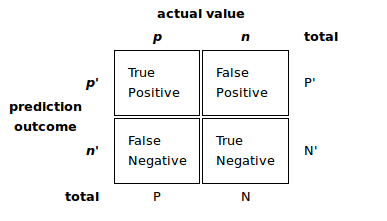
\includegraphics[width=3.0in]{FourValues}
\caption{Confusion matrix}\label{ConfusionMatrix:1}
\end{figure} 

%An example to understand these four values: the detection of positives and negatives.

Take a simple example to understand these four values. 
If ten people go to the hospital to detect whether they have a disease. Actually, five of them are positive, others are negative. So the actual values of positive are five and actual values of negative are also five. But by testing, six are positive, which is called the prediction outcome of positive. Among them, four are really positive, and the two other people are negtive. So the four people are true positive and the two are false positive. As we know, one people is not tested but actually he is positive , so this is called false negtive. And other three people are negative and the test results are right, so they are called true negative. 

\begin{table}
\centering\caption{}
\begin{tabular}{|r|c|c|}
\hline
&Actual Pos=5&Actual Neg=5\\
\hline
Prediction Pos=6&TP=4&FP=2\\
\hline
Prediction Neg=4&FN=1&TN=3\\
\hline
\end{tabular}
\end{table}

\section{ROC space and PR space}

\subsection{Structure of the two spaces}
%The illustration of x-axis and y-axis in ROC space: format, meaning.
In ROC space, one plots the False Positive Rate (FPR) on the x-axis and the True Positive Rate (TPR) on the y-axis. These two values can be caculated by the formula (\ref{eq:FPR}) and formula (\ref{eq:TPR}). TP, FP, FN, TN are introduced in the section above. The FPR measures the fraction of negative examples that are misclassified as positive. The TPR measures the fraction of positive examples that are correctly labeled. Both of them range from $0$ to $1$. It is obvious that we want to get a big TPR and a small FPR. So if the point is closer to top left, it may have better result. Figure \ref{ROC:1} is a graph of ROC space.

\begin{equation}\label{eq:FPR}
FalsePositiveRate=\frac{FP}{FP+TN}
\end{equation}
\begin{equation}\label{eq:TPR}
TruePositiveRate=\frac{TP}{TP+FN}
\end{equation}

\begin{figure}[!ht]
\centering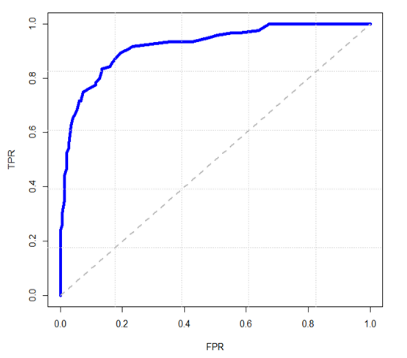
\includegraphics[width=3.0in]{ROC}
\caption{ROC}\label{ROC:1}
\end{figure} 

%The illustration of x-axis and y-axis in PR space: format, meaning. 
In PR space, one plots Recall on the x-axis and Precision on the y-axis. These two values can be caculated by formula (\ref{eq:Recall}) and formula (\ref{eq:Precision}). Recall is the same as TPR, whereas Precision measures the fraction of examples classified as positive that are true positive. Both of them range from $0$ to $1$. It is obvious that we want to get a big Recall and a big Precision. So if the point is closer to top right, it may have better result. Figure \ref{PR:1} is a graph of ROC space.

According to these formulas, the denominators of TPR and Recall are the actual value of positive and the denominator of FPR is the actual value of negative indeed. So they are unrelated with the results of prediction. Only the denominator of Precision value is related to the prediction.
\begin{equation}\label{eq:Recall}
Recall=\frac{TP}{TP+FN}
\end{equation}
\begin{equation}\label{eq:Precision}
Precision=\frac{TP}{TP+FP}
\end{equation}

\begin{figure}[!ht]
\centering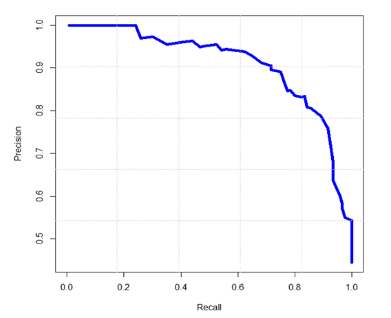
\includegraphics[width=3.0in]{PR}
\caption{PR}\label{PR:1}
\end{figure} 

\subsection{Points in ROC space and PR space}

\subsubsection{Caculation of the coordinates}
%Explaination of the caculation with the example in section $2$. 
The confusion matrix can be used to caculate a point in either ROC space or PR space. Let's go back to the first example. The values of TP, FP, FN, TN we obtained are 4, 2, 1, 3 respectively. So the TPR, FPR values in ROC space and the Recall, Precision values in PR space can be caculated according to the formula. $FPR=\frac{2}{5}$, $TPR=R=\frac{4}{5}$, $R=\frac{4}{5}$, $P=\frac{4}{6}$. By caculating, we get the point ($\frac{2}{5}$,$\frac{4}{5}$) in ROC space and the point ($\frac{4}{5}$,$\frac{2}{3}$) in PR space.

\subsubsection{The one-to-one correspondence between the points in these two spaces}
%Theorem and proof.
In this part, we will introduce the relationship between the points in these two spaces and prove it.

Relationship: for a given dataset of positive and negative examples, there exist a one-to-one correspondence between the points in ROC space and PR space, such that the points contain exactly the same confusion matrices, if Recall is not zero \cite{3:article}.

\begin{proof} Note that given the point in PR space and the dataset of fixed positive and negtive examples, TP will be fixed according to the formula (\ref{eq:Recall}). And the FP is also fixed as TP is fixed according to the formula (\ref{eq:Precision}). Then it is known that a point in PR space defines a unique confusion matrix. And unique point in ROC space can be obtained according to this confusion matrix.

But when Recall is zero, we can only make a conclusion that the TP is zero and then Precision is zero while FP can't be fixed. So the confusion matrix is not unique and the point in ROC space is not unique.

Consequently, we have a one-to-one mapping between confusion matrices and points in PR space. This implies that we also have a one-to-one mapping between points (each defined by a confusion matrix) in ROC space and PR space.
\end{proof}
\subsection{Curves in ROC space and PR space}
%Generation of the curve: different thresholds.
When got one point from the calculation, the PR graph or ROC graph can only show one point. The curve can be obtained as its discrimination threshold is varied.
\subsubsection{Relationship between these two curves}
\begin{itemize}
\item Domination relationship 

For a fixed number of positive and negative examples, one curve dominates a second curve in ROC space if and only if the first dominates the second
in PR space. The meaning of one curve dominates another is that all other curves are beneath it or equal to it without intersection \cite{3:article}.

\begin{proof} If a curve dominates in ROC space then it dominates in PR space. Proof by contradiction. Suppose we have curve I and curve II such that curve I dominates in ROC space, yet, once we translate these curves in PR space, curve I no longer dominates. Since curve I does not dominate in PR space, there exists some point A on curve II such that the point B on curve I with identical Recall has lower Precision. In other words, $Precision(A)>Precision(B)$ yet $Recall(A) = Recall(B)$. Since $Recall(A) = Recall(B)$ and Recall is identical to TPR, we have that $TPR(A) = TPR(B)$. Since curve I dominates curve II in ROC space $FPR(A) ≥ FPR(B)$. Remember that total positives and total negatives are fixed and since $TPR(A) = TPR(B)$. We now have $TPA = TPB$ and thus denote both as TP. Remember that $FPR(A)\ge FPR(B)$ and  
\begin{equation}\label{eq:FPR}
FalsePositiveRate=\frac{FP}{Total Negatives}
\end{equation}    
 This implies that $FPA \ge FPB$ because
\begin{equation}\label{eq:P}
Precision=\frac{TP}{TP+FP}
\end{equation}

We now have that $Precision (A)\le Precision (B)$. But this contradicts our original assumption that $PRECISION (A) >PRECISION (B)$. So the assumption is wrong and the curve I should also dominates curve II in PR space.

Similarly, if a curve dominates in PR space then it dominates in ROC space, we don't give the proof as it is similar to the proof above.
\end{proof}
\item The situation of two curves intersect 

When the two curves intersect, the proof above can't work as the step $FPR(A)\ge FPR(B)$ can't be guaranteed in the whole space. But if choosing a range which one curve dominates the other, the same conclusion can be obtained. In other words, if one curve dominates another in an certain range (refers to the abscissa) of PR space, then it will dominate in this range (refers to the ordinage) of ROC space. 

We prove it by an experiment.

Define two curves \ref{pr:1} in PR space and each curve has five certain points. The two curves have two intersections at point $(0.2,0.7)$ and $(0.6,0.4)$. When abscissa ranges from $0$ to $0.2$ and from $0.6$ to $0.8$, the blue curve dominates. And the red dominates from $0.2$ to $0.6$. When transforming these curves to ROC space \ref{roc:1}, the blue curve dominates at the same range in ordinate. Note that the abscissa in PR space and the ordinate in ROC space have same meaning.

So if one curve dominates another in an certain range (refers to the abscissa) of PR space, then it will dominate in this range (refers to the ordinage) of ROC space. 
 
\begin{figure}[!ht]
\begin{minipage}[t]{0.5\textwidth}
\centering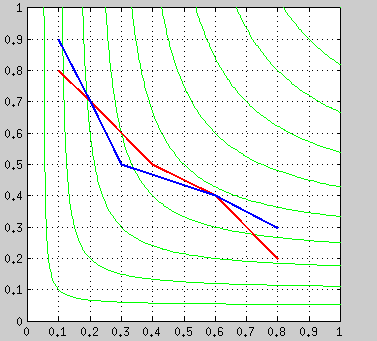
\includegraphics[width=2.0in]{PR_test1}
\caption{Curves in PR space}\label{pr:1}
\end{minipage}
\begin{minipage}[t]{0.5\textwidth}
\centering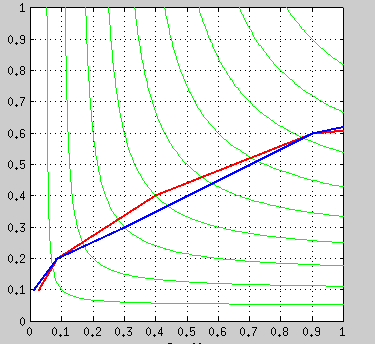
\includegraphics[width=2.0in]{ROC_test1}
\caption{Curves in ROC space}\label{roc:1}
\end{minipage}
\end{figure}
\end{itemize}

\subsubsection{The achievable PR curve}

\begin{enumerate}
\item A corollary
\newtheorem{corollary}{corollary} %定理
\begin{corollary}
Given a set of points in PR space, there exists an achievable PR curve that dominates the other valid curves that could be constructed with these points.
\end{corollary}
Before proof, it is necessary to introduce the concept of convex hull. Convex hull is a computational geometry in the concept. For a given set of points on a two-dimensional plane, convex hull is the convex polygons which is composed by connecting the dots outermost.  Given a set of points in ROC space, the convex hull must meet the following three criteria:
\begin{itemize}
\item Linear interpolation is used between adjacent points.
\item No point lies above the final curve.
\item For any pair of points used to construct the curve, the line segment connecting them is equal to or below the curve.
\end{itemize}

In PR space, there exists an analogous curve to the convex hull in ROC space, which we call the achievable PR curve.

\begin{proof} First, convert the points in PR space into ROC space, and construct the convex hull of these points in ROC space. By definition, the convex hull dominates all other curves that could be constructed with those points when using linear interpolation between the points. Thus converting the points of the ROC convex hull back into PR space will yield a curve that dominates in PR space. The achievable PR curve will exclude exactly those points beneath the convex hull in ROC space.

\begin{figure}[!ht]
\begin{minipage}[t]{0.5\textwidth}
\centering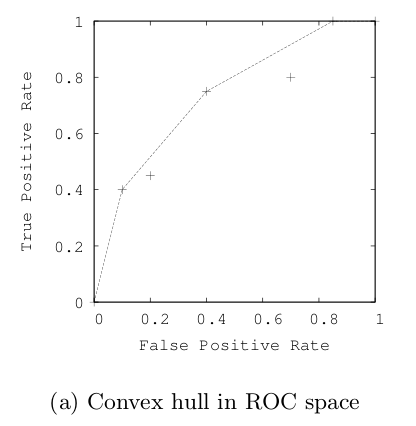
\includegraphics[width=2.6in]{convex1}
\end{minipage}
\begin{minipage}[t]{0.5\textwidth}
\centering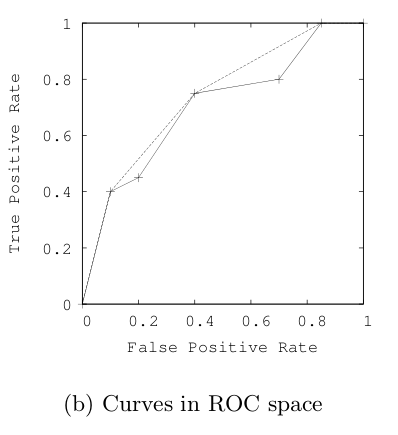
\includegraphics[width=2.5in]{convex2}
\end{minipage}
\end{figure}
\begin{figure}[!ht]
\centering
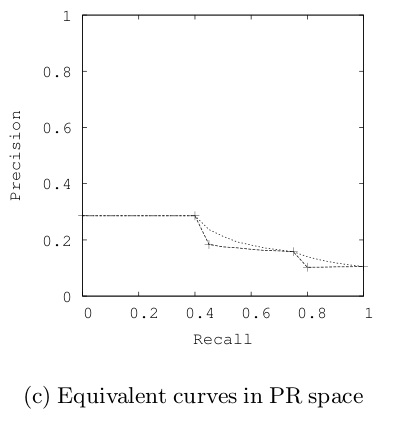
\includegraphics[width=3.0in]{convex3}
\caption{Convex hull}\label{convex_hull}
\end{figure} 

Figure \ref{convex_hull} is graphs about the convex hull. The dashed line in Figure (a) is the convex hull of the fixed points in ROC space. And the the solid line in Figure (b) is the acutual curve. When transformed into PR space, these two curves will become those in Figure (c). The dashed line in Figure(c) is the achievable PR curve which dominates all other valid curves.
\end{proof}

\item Interpolation in PR space

Suppose there are two points which are far apart in PR space. It may yield an over-optimistic estimate of performance when just connecting them to construct PR curve\cite{3:article}. As the level of Recall varies, the Precision does not necessarily change linearly due to the fact that $FP$ replaces $FN$ in the denominator of the Precision. Then it is necessary to interpolate between points. Corollary above shows how to find the achievable PR curve by simply converting the analogous ROC convex hull; this yields the correct interpolation in PR space. However, a curve consists of infinitely many points, and thus we need a practical, approximate method for translation. We expand here on the method proposed by Goadrich et al. (2004) to approximate the interpolation between two points in PR space \cite{8:article}.

Remember that any point A in a Precision-Recall space is generated from the underlying true positive ($TP_A$ ) and false positive ($FP_A$) counts. Suppose there are two points, A and B which are far apart in PR space. To find some intermediate values, it is necessary to interpolate between their counts $TP_A$ and $TP_B$ , and $FP_A$ and $FP_B$ . Find out how many negative examples it takes to equal one positive, or the local skew, defined by $\frac{FP_B-FP_A}{TP_B-TP_A}$ . Now create new points $TP_A+x$ for all integer values of $x$ such that $1 \le x \le TP_B − TP_A$, i.e. $TP_A +1, TP_A +2, ..., TP_B −1$,and calculate corresponding $FP$ by linearly increasing the false positives for each new point by the local skew. The resulting intermediate Precision-Recall points will be $(\frac{TP_A +x}{Total Positive},\frac{TP_A +x}{TP_A+x+FP_A+\frac{FP_B-FP_A}{TP_B-TP_A}x})$.

For example, suppose we have a dataset with 20 positive examples and 2000 negative examples. Let $TP_A=5$, $FP_A=5$, $TP_B=10$, and $FP_B=30$. Table below  shows the proper interpolation of the intermediate points between A and B, with the local skew of 5 negatives for every 1 positive. Notice how the resulting Precision interpolation is not linear between $0.50$ and $0.25$.
\begin{center}
\begin{tabular}{|c|c|c|c|c|}
\hline
 &TP&FP&REC&PREC\\
\hline
A&5&5&0.25&0.500\\
.&6&10&0.30&0.375\\
.&7&15&0.35&0.318\\
.&8&20&0.40&0.286\\
.&9&25&0.45&0.265\\
B&10&30&0.50&0.250\\
\hline
\end{tabular}
\end{center}
 
\end{enumerate}

\subsubsection{The advantages of PR curve}
%The illustration of  changes on the  P, R, FPR, TPR  if  the given data have a big positive value or negtive value respectively. In this way, explain the insensitivity of ROC.
As we know, both of the two curves can evaluate the performance, but what is the difference between them? 

At the beginning of this document, we simply say that PR curve can also make a fair evaluation when the given tasks have a large skew, while ROC curve can't do that better. Now, we will explain it in details.

We have known that the Recall value in PR curve and the TPR value in ROC curve is equivalent, so it is unnecessary to consider them. Think about the Precision value and FPR value in formula (\ref{eq:Precision}) and formula (\ref{eq:FPR}). We have discussed about the denominators of abscissa and ordinate in these two values in section 3.1, and say that the denominator of FPR is the actual value of negative and it is unrelated with the result of prediction while the Precision value is related.

If the number of negative examples greatly exceeds the positive examples in the given dataset, the denominator of FPR will be exceedingly large. And when the FP has a large change, it only can lead to a small change in FPR. So the points in ROC will be close to the y-axis as the value of FPR is very small. On the contrary, if given lots of positive examples, the FPR value is close to $1$ and hardly changes any more. In this case, ROC doesn't sensitive to the results we get from an algorithm if the given samples have a certain degree of particularity. This is not what we want as it can't evaluate our algorithm fairly. While Precision value only gets a ratio between TP and prediction positives and it doesn't care how many positive or negtive examples it originally has. So PR curve has a fairer evaluation compared to ROC curve.

Looking at PR curves can expose differences between algorithms that are not apparent in ROC space. Sample ROC curves and PR curves are shown in \ref{comparison} respectively. These curves, taken from the same learned models on a highly-skewed cancer detection dataset, highlight the visual difference between
these spaces. The goal in ROC space is to be in the upper-left-hand corner, and when one looks at the ROC curves they appear to be fairly close to optimal. In PR space the goal is to be in the upper-right-hand corner, and the PR curves show that there is still vast room for improvement.

\begin{figure}[!ht]
\centering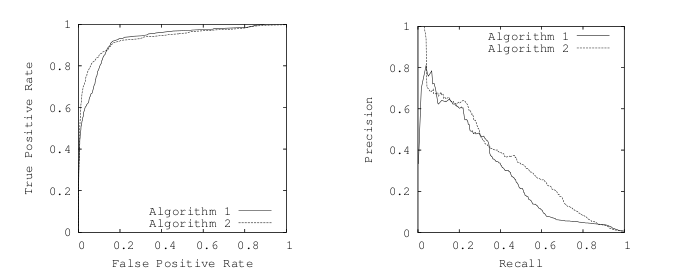
\includegraphics[width=5.0in]{compared}
\caption{Comparison of ROC and PR}\label{comparison}
\end{figure} 




\section{Evaluation  of ROC and PR curves}
%The reason why evaluating them.
From the curve, We can only obtain intuitive results. But if two curves are intersect in one PR or ROC space, it is hardly know which curve is better. So it is necessary to use some quantitative analysis to evaluate them.
\begin{description}
\item[ROC] People generally use Area under ROC curve (AUC) to evaluate ROC curve. As the name implies, the AUC value is the size of the area under the ROC curve. Typically, the AUC values range from $0.5$ to $1.0$, and the larger AUC represents the better Performance.
\item[PR] Precision-Recall
\begin{enumerate}
\item F measure \cite{4:article} \cite{7:misc}: $F=2PR/(P+R)$. We can caculate the optimal F measures of curves to evaluate. The larger the F value, the better the curve.
\item Average precision(AP) \cite{3:article} \cite{5:article}. Actually, it is the area under the PR curve. The larger the AP value, the better the curve. 
\end{enumerate}
\end{description}

%\item 候晓迪 CVPR2013

\section{Evaluation of image segmentation using ROC and PR curves}
%Relationship between original image, Ground Truth image and processed image.
The ROC curve and PR curve can also apply to the field of image segmentation. We can evaluate the segmentation algorithm by observing the trend of the two curves. Given an original image, it is necessary to transform it to Ground Truth image (short for GT) which is obtained by artificial matting typically. The GT is used to compare with the image processed by segmentation algorithm, as it is the most accrurate segmention way until now. When using ROC or PR curves to evaluate, we need to change the format of GT and processed image to binary images. In this case, they can be compared easily.

\subsection{The procedure to construct the ROC and PR curves}
Take an example of constructing the ROC and PR curves in the field of image segmentation to understand these two curves better.  

\begin{itemize}

\item Transformation of the GT: %choice of the threshold.

Table 2 is the given GT image. As we known above, it is necessary to change the format if it isn't a binary image. But how to choose the threshold to transform it from a gray-scale image to a binary image (If the GT image is a color image, we need to transform it to the gray-scale image first)? In BSDS500(one dataset of image segmentation which offer an evaluation method), they offer two methods. One is an fixed threshold for all images in the dataset, calibrated to provide optimal performance on the training set. They call it the optimal dataset scale(ODS). And another is the optimal threshold seleted on per image. They call it optimal image scale(OIS), one natually obtains even better segmentations\cite{4:article}.
\begin{table}[h]
\centering
\begin{minipage}[t]{0.25\linewidth}
\caption{}
\begin{tabular}{|c|c|c|c|}
\hline
0&0&0&0\\
\hline
0&1&1&0\\
\hline
0&1&1&0\\
\hline
0&0&0&0\\
\hline
\end{tabular}
\end{minipage}
\begin{minipage}[t]{0.25\linewidth}
\caption{}
\begin{tabular}{|c|c|c|c|}
\hline
128&0&0&0\\
\hline
0&255&0&0\\
\hline
0&64&192&0\\
\hline
0&0&0&64\\
\hline
\end{tabular}
\end{minipage}
\end{table}

\item Transformation of the processed image: %normalization
Table 4 is the processed image. Normalize the processed image in order to have a contrast with the GT image.
\begin{table}[ht]
\centering
\caption{}
\begin{tabular}{|c|c|c|c|}
\hline
0.5&0&0&0\\
\hline
0&1&0&0\\
\hline
0&0.25&0.75&0\\
\hline
0&0&0&1\\
\hline
\end{tabular}  
\end{table}

\item Caculate Recall, Precision, FPR, TPR: 
%We can get different points, line them and get the curve.

Then caculate the values of Recall, Precision, FPR, TPR.

If choose $0.25$ as the threshold, all values biger than $0.25$ will turn to be $1$ for the processed image, and the left will turn to be $0$. Then we get the table 5.
\begin{table}[h]
\centering
\caption{}
\begin{tabular}{|c|c|c|c|}
\hline
1&0&0&0\\
\hline
0&1&0&0\\
\hline
0&1&1&0\\
\hline
0&0&0&1\\
\hline
\end{tabular} 
\end{table}


So the $FPR=\frac{2}{12}=\frac{1}{6}$,$TPR=R=\frac{3}{4}$, $Recall=\frac{3}{4}$, $Precision=\frac{3}{5}$. We can obtain the point $(1/6,0.75)$ in ROC space and the point $(0.75,0.6)$ in PR space.

In this case, three points will be obtained in ROC space, $(1/6,0.75)$, $(1/12,0.5)$, $(0,0.5)$, and three points in PR space, $(0.75,0.6)$, $(0.5,2/3)$, $(0.5,0.4)$. Line them and the ROC curve or PR curve is formed.
\end{itemize}

\subsection{Method to get one PR curve in BSDS500}
%The introduction of the method to get one curve in BSDS.
One image will form one curve, but one dataset may have hundreds of images, they will form hundreds of curves. How can one curve represent all of them?

In BSDS500, they use the whole TP to divide the whole TP and FP as the Precision value and the whole TP divide the whole TP and FN as the Recall value \cite{4:article}.

For example, Table 6 and Table 8 are GT images, and Table 7 and Table 9 are processed images. If choose 0.5 as the threshold, then the caculation of the point in PR space is below:
$Recall=\frac{2+2}{4+4}=0.5$, $Precision =\frac{2+2}{3+4}=\frac{4}{7}$.
So we obtain one point at the the threshold of 0.5. In this case, one PR curve of lots of images can be obtained. In other words, the whole Presion and Recall value should be caculate by the formula \ref{eq:whole_Recall} and \ref{eq:whole_Precision}.
\begin{table}[!ht]
\begin{minipage}[t]{0.17\linewidth}
\caption{}
\begin{tabular}{|c|c|c|c|}
\hline
0&0&0&0\\
\hline
0&1&1&0\\
\hline
0&1&1&0\\
\hline
0&0&0&1\\
\hline
\end{tabular} 
\end{minipage}
\begin{minipage}[t]{0.33\linewidth}
\caption{}
\begin{tabular}{|c|c|c|c|}
\hline
0.5&0&0&0\\
\hline
0&1&0&0\\
\hline
0&0.25&0.75&0\\
\hline
0&0&0&0.25\\
\hline
\end{tabular} 
\end{minipage}
\begin{minipage}[t]{0.2\linewidth}
\caption{}
\begin{tabular}{|c|c|c|c|}
\hline
1&1&0&0\\
\hline
1&1&0&0\\
\hline
0&0&0&0\\
\hline
0&0&0&0\\
\hline
\end{tabular} 
\end{minipage}
\begin{minipage}[t]{0.01\linewidth}
\caption{}
\begin{tabular}{|c|c|c|c|}
\hline
0.6&0&0&0\\
\hline
0.8&0.4&0&0\\
\hline
0&0.7&0.8&0\\
\hline
0&0&0&0\\
\hline
\end{tabular} 
\end{minipage}
\end{table}

\begin{equation}\label{eq:whole_Recall}
Recall=\frac{\displaystyle\sum_{i=1}^n(TP_i)}{\displaystyle\sum_{i=1}^n((TP_i)+(FN_i))}
\end{equation}
\begin{equation}\label{eq:whole_Precision}
Precision=\frac{\displaystyle\sum_{i=1}^n(TP_i)}{\displaystyle\sum_{i=1}^n((TP_i)+(FP_i))}
\end{equation}

\subsection{The reason why BSDS choose PR curve instead of ROC curve}
We have introduced the advantages of PR curve in section $3.3.2$. When involved to the field of image segmentation, we can think in this way. It is a commonly method to use segmentation algorithms to extract the edge of objects. And the use of ROC or PR curve to evaluate the results of algorithms is necessary. The edge has only one pixel width, and when using an algorithm to detect the contour, the amount of pixels we get actually is very small. If the contour pixels represent positive samples, then the negtive samples are very large. So the FPR value is inaccurate to a certain extent because it is insensitive to the FP value. And this is not we want. While Precision value is only evaluating the ratio between TP and prediction positives, it doesn't care the amount of positive examples or negative examples it originally has. And it will also change heavily when TP or FP value changes. So it is more sensitive to the results of contour detection. This is why BSDS doesn't choose ROC curve to evaluate their algorithms\cite{6:misc}.  



\section{Experiments}

\subsection{A matlab function to compute and plot ROC and PR curves}
There is a function of Precision-Recall and ROC curves called prec\_rec.m created by Stefan Schroedl. It is used for caculating and ploting PR and ROC curves for binary classification tasks initially.
You can refer it from $https://github.com/zhenglab/ROC\_PR.git$.

\subsection{ROC and PR curves applied to the field of image processing}
When using the program above to deal with image, it is necessary to do some pretreatment. The program below is a function about the pretreatment of image and we can obtain the ROC and PR curves only by inputting the compared image. The figure 6, 7, 8, 9 are original image(bmp format), GT image(bmp format), processed image(png format), and the result respectively. 
\lstinputlisting{../programs/prec_rec_img_seg/prec_rec_img_prepro.m}
\begin{figure}[!ht]
\centering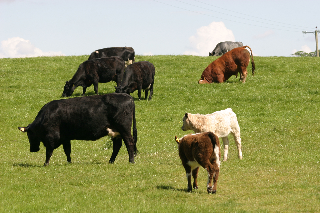
\includegraphics[width=2.5in]{1_11_s1.png}
\caption{Original image}
\end{figure} 

\begin{figure}[!ht]
\begin{minipage}[t]{0.5\textwidth}
\centering
\includegraphics[width=2.5in]{1_11_s_GT.png}
\caption{GT}
\end{minipage} 
\begin{minipage}[t]{0.5\textwidth}
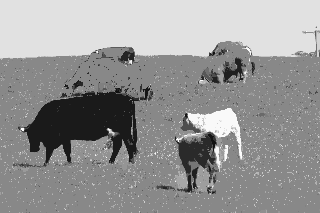
\includegraphics[width=2.5in]{1_11_s.png}
\caption{Processed image}
\end{minipage}
\end{figure} 

\begin{figure}[!ht]
\centering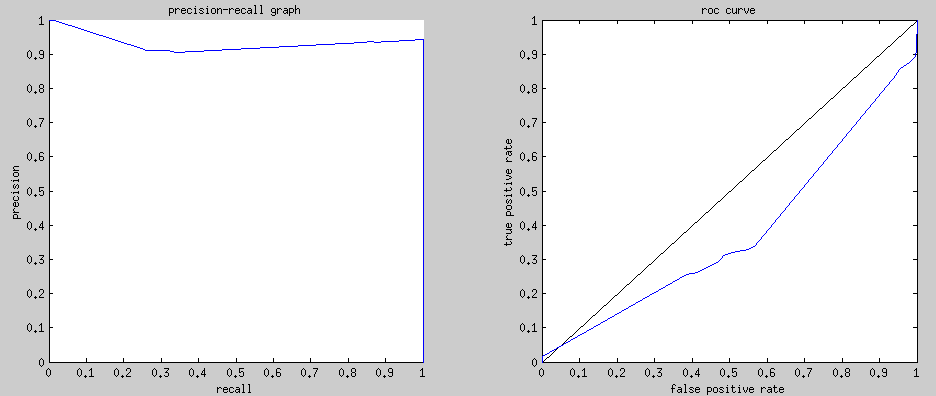
\includegraphics[width=5.0in]{image_seg}
\caption{result}
\end{figure} 

By observing the result, it is hardly to say whether it is right or not as the amount of pixels in image is so large that caculating the result is impossible to some extent. So I design an image with $32\times32$ pixels to see the result. Figure 10 and 11 are GT and Processed image respectively. And the result is what we want.
\lstinputlisting{../programs/prec_rec_img_seg/create_img_input.m}

\begin{figure}[!ht]
\begin{minipage}[t]{0.5\textwidth}

\includegraphics[width=2.0in]{creat2.png}
\caption{GT}
\end{minipage}
\begin{minipage}[t]{0.5\textwidth}
\centering
\includegraphics[width=2.0in]{creat1.png}
\caption{Processed image}
\end{minipage}
\end{figure} 
\begin{figure}[!ht]
\centering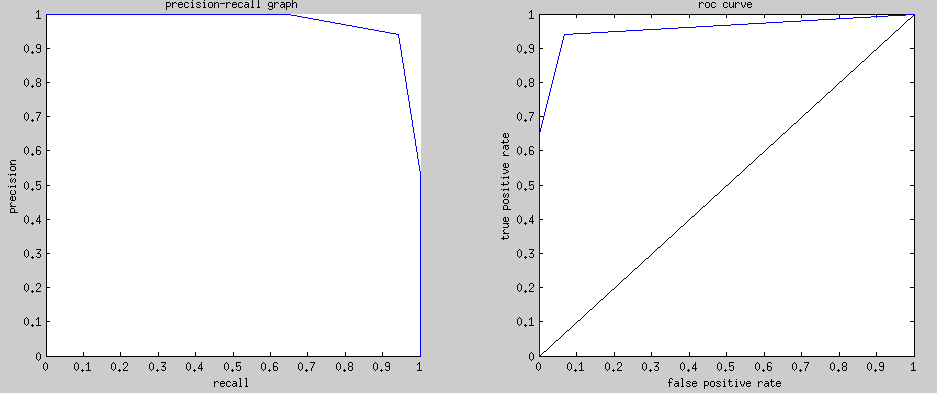
\includegraphics[width=5.0in]{result2.png}
\caption{result}
\end{figure}

\subsection{Two curves intersect}

The experiment in section $3.3.1$ is designed by myself. In order to illustrate its validity, I compared the results obtained by the $prec\_rec.m$ function and the program written by myself. The experiment shows that they have the same results. The first program is written by myself and the second uses the $prec\_rec.m$ function. The figure 13, 14 and figure 15 are their result respectively. (I modified some parts in $prec\_rec.m$, for example, the $\ge$is changed as $>$ in line $134$, and the output using plot function is also changed.)

\lstinputlisting{../programs/PR_ROC_intersect/my_test/two_points.m}
\lstinputlisting{../programs/PR_ROC_intersect/prec_rec/input.m}

\begin{figure}[!ht]
\begin{minipage}[t]{0.5\textwidth}
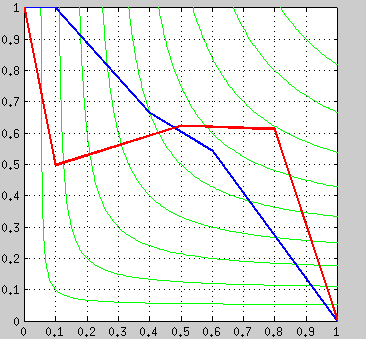
\includegraphics[width=2.5in]{intersect2.png}
\caption{PR}
\end{minipage}
\begin{minipage}[t]{0.5\textwidth}
\centering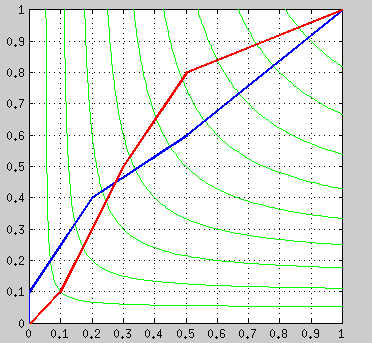
\includegraphics[width=2.5in]{intersect1.png}
\caption{ROC}
\end{minipage}
\end{figure}

\begin{figure}[!ht]
\centering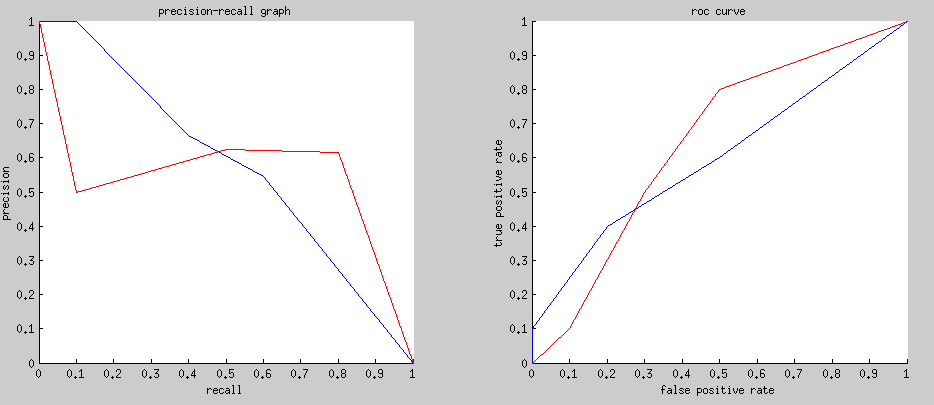
\includegraphics[width=5.0in]{intersect3}
\caption{PR and ROC}
\end{figure} 

\subsection{The sensitivity of PR curve}

We have talked about the advantages about PR curve above as it is more sensitive than ROC curve. The experiment below proofs it. We obtained different PR curves and ROC curves as the amount of actual positive changes. By looking at the results (I just choose three results to see), it is easily to know that PR curves change largely while ROC curves change little. Consequently, PR curve is more sensitive to the samples and then we can easily know the differences between the analogous samples from PR curve.   

\lstinputlisting{../programs/PR_advantages/input.m}
\begin{figure}[!ht]
\centering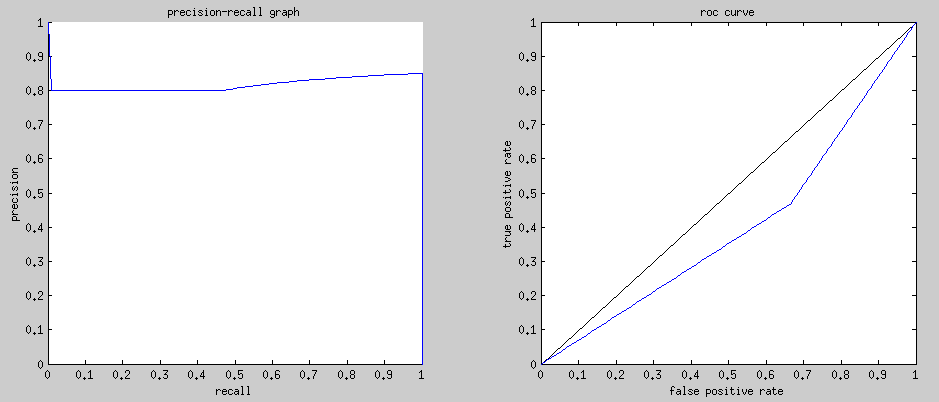
\includegraphics[width=5.0in]{compare1}
\end{figure} 
\begin{figure}[!ht]
\centering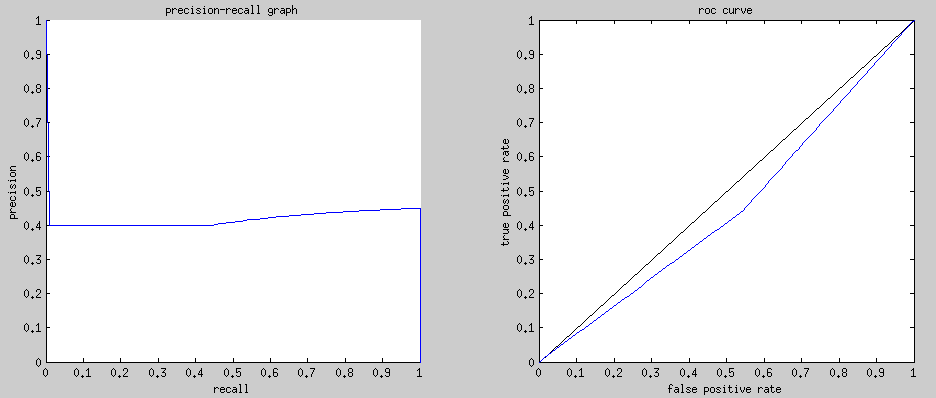
\includegraphics[width=5.0in]{compare2}
\end{figure} 
\begin{figure}[!ht]
\centering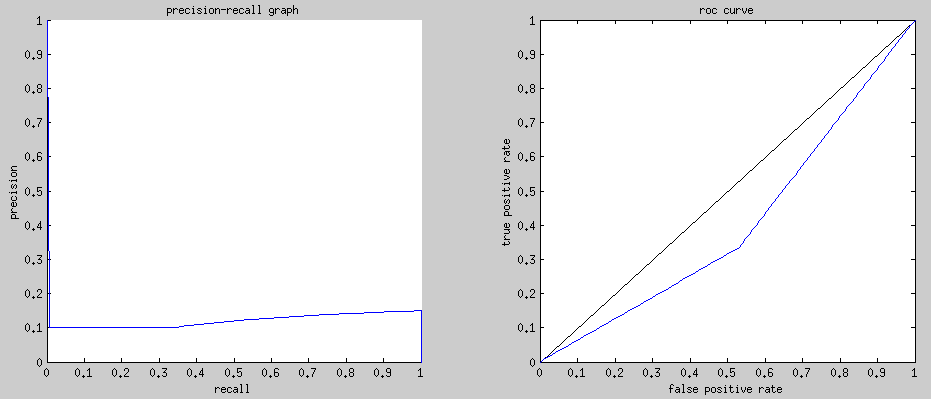
\includegraphics[width=5.0in]{compare3}
\end{figure} 

\bibliographystyle{plain}
\bibliography{ROC_PR}


\end{document}



